\section{{\sys} Algorithm}
\label{sec:algorithm}

\subsection{Overview}
\label{sec:algorithm_overview}

\begin{figure*}[!ht]
\centering
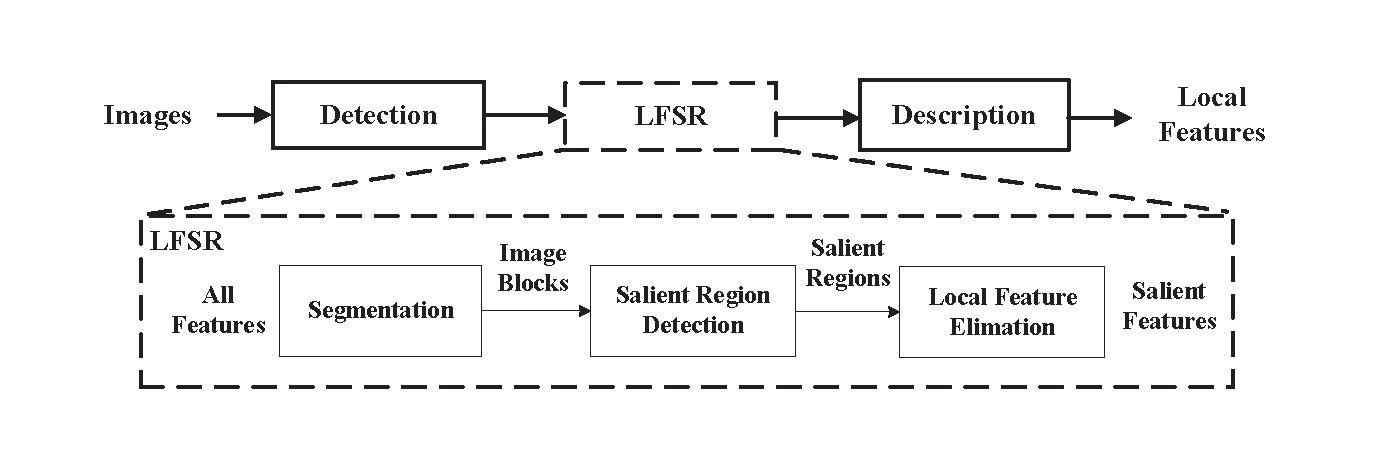
\includegraphics[width=4.5in]{images/fig-overview.eps}
\caption{An overview of {\sys}}
\label{fig:overview}
\end{figure*}

The basic motivation of {\sys} is to design a salient region detection algorithm, which can be used to optimize the obstacles of {\lfea}s and is easy to combined with them. Based on the observations in Section~\ref{subsec:observation}, we design and implement a local feature based salient region algorithm~({\sys}), which is efficient and easy to be combined with {\lfea}s.    

As shown in Figure \ref{fig:overview}, {\sys} works as a filter just between detection stage and description stage of a typical {\lfea}, where the input of {\sys} is detected feature points and its output is the sets of concerned feature points for computing feature vectors. There exist two major stages in our algorithm.
\begin{inparaenum}[\itshape a\upshape)]
\item First, a segmentation step is performed on all local features to identify and partition multiple salient region in an image. 
\item Second, for each image segmentation, {\sys} computes that segmentation's salient region individually based on the distribution information of the local feature points in it.
\end{inparaenum}


\subsection{Local Feature Based Segmentation}
\label{sec:algorithm_segmentation}

According to Observation~\ref{itm:observation_2}, an image may include several salient regions, which form multiple clusters of local features. We solve this problem by using a simple segmentation algorithm to divide the image into several blocks based on the distribution of local features. It scans along both the x axis and the y axis. In each scan, a cut-point may be found under the following two constraints:

\squishlist
\item \textit{No local feature could be divided into multiple parts.} In {\lfea}s, scale information is computed to guaranteed scale invariant. Therefore, a local feature point is used to represent a region with a radius that equals its scale as shown in Figure~\ref{fig:segmentation}. When the image is partitioned, no segmentation should across the region that a feature point representing.

\item \textit{The cut point should not locate far away form the center.} Each scan is performed from the region center. When the scan goes far, for example 1/4 of the region width, the scan stops and declares that there is no valid cut in that scan. This constraint attends to keep segmentation balanced and avoid too large or too small regions.
\squishend

A typical segmentation is shown in Figure~\ref{fig:segmentation}. The segmentation is started from the center of each axis, e.g. the dot lines in the figure. When a cut-point satisfying the above two constraints is found, The algorithm stops scanning and takes that cut-point as a valid image segmentation, e.g. the solid lines in the figure. After scanning on both the x axis and the y axis, at most four image regions are found in one segmentation.

\begin{figure}[!ht]
\centering
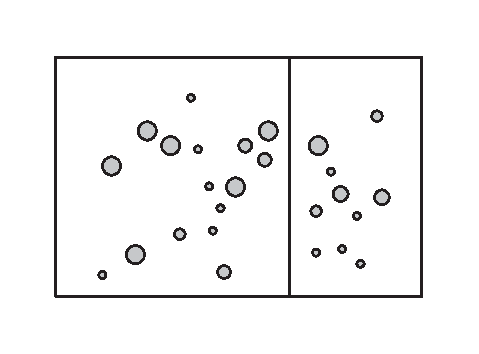
\includegraphics[width=2.1in]{images/fig-segmentation.eps}
\caption{Segmentation by scanning along both the x-axis and y-axis and starting from the dot lines and stops on the solid lines.}
\label{fig:segmentation}
\end{figure}

Then this kind of segmentation will be performed recursively on each image regions. And a recursive segmentation should stop when the following situations are satisfied:

\squishlist
\item \textit{No valid cuts are found.} When no valid cuts following the above two constraints are found, for example a scan exceeds its distance limit, on both x-axis and y-axis of a region, we should regard this region as a whole object and stop performing segmentation on it.

\item \textit{Too few features exist in a region.} Some found regions may have no local feature or just a few features, such as one or two local features, like gray regions in Figure~\ref{fig:segmentation-2}. These regions will be marked as invalid, because they cannot hold one whole object, and no further computation will be performed on them.

\item \textit{The number of segmentations exceeds the limitation.} It's possible that the recursive segmentation becomes too deep if there exist many dispersive points in that region. And actually it makes no sense to perform segmentation on these points, since they cannot be regarded as valid objects individually.

\squishend

\begin{figure}[!ht]
\centering
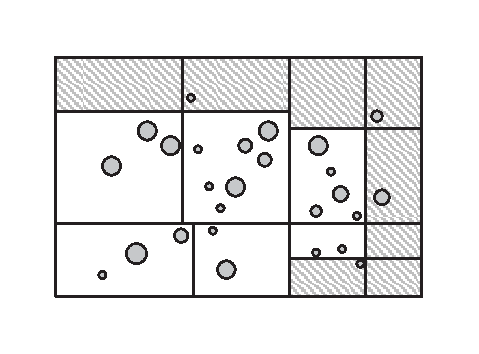
\includegraphics[width=2.1in]{images/fig-segmentation-2.eps}
\caption{Valid and invalid regions after two runs of segmentations. White regions are valid and gray regions are invalid.}
\label{fig:segmentation-2}
\end{figure}


According to our evaluation, in most cases two runs of segmentation are just enough, since almost no image has more than sixteen major objects. Thus, it's possible to simplify this processing by performing segmentation only twice in realistic scenarios.

\subsection{Salient Regaion Detection}
\label{sec:algorithm_detection}

As discussed in Section~\ref{sec:algorithm_overview}, a precise salient region detection is not suitable for local feature reduction in terms of processing speed and accuracy. Thus, {\sys} employs geometric meaning of local features to compute approximate salient regions.

According to Observation~\ref{itm:observation_1}, the local features in one salient region locate near to each other while noise or unimportant feature points locate far away from them. To simplify this problem, we regard the geometric center of feature points as the center of a salient region. Thus, the region center can be calculated based on the following equation:

{\begin{equation} \label{eq:center}
\left({x}_{c},{y}_{c} \right) = \frac{\sum_{i}^{N}\left({x}_{i},{y}_{i} \right)}{N}
\end{equation}}

Where $\left({x}_{c},{y}_{c} \right)$ means the geometric center of each local feature $\left({x}_{i},{y}_{i} \right)$ in that image segmentation.

After locating the center, we build the final salient regions by expanding the region as a rectangle with a particular width-length ratio. This ratio should be consistent with the distribution of local features, since local features always locate following the shape of target objects. Approximately, this ratio can be considered to equal to the ratio of the dispersion degree on x-axis and y-axis. For example, the bigger dispersion degree of local features on x-axis is, the bigger width-length ratio we will get. To compute the ratio of feature dispersions, we can divide the standard deviation of local feature position on x-axis by on y-axis:

{\begin{equation} \label{eq:ratio}
ratio = \sqrt{\frac{\sum_{i}^{N}\left ( x_{i}-x_{c} \right )^{2}}{\sum_{i}^{N}\left ( y_{i}-y_{c} \right )^{2}}}
\end{equation}}

Where $x_{i}$ and $y_{i}$ is a feature's position, while $x_{c}$ and $y_{c}$ is the center position computed by Equation~\ref{eq:center}. To get the final salient region, {\sys} grows the region size until the amount of local feature in it exceeds a desirable number, for example 50 percent of the original local features. As discussed in Observation \ref{itm:observation_3}, this threshold is important for providing a large enough salient region to avoid filtering local features on objects' edges and corners. In our evaluation, we find a ratio about 40\% is proper for most cases.

Combined with segmentation discussed in Section~\ref{sec:algorithm_segmentation}, the processing results will provide several candidate regions. According to Observation \ref{itm:observation_2}, we pick up the candidate regions that have at least 2 local features inside and regard them as the final salient regions.

\subsection{Local Feature Elimination}
\label{sec:algorithm_elimation}

With the knowledge of salient regions in an image, all features locate inside salient regions are kept for further computation, and all other features outside are just dropped. As a result, we get much fewer salient features in the local feature description stage, which can help to improve the whole algorithm's efficiency obviously.

